% Created 2025-11-04 火 17:16
% Intended LaTeX compiler: xelatex
\documentclass[11pt]{article}
\usepackage{graphicx}
\usepackage{longtable}
\usepackage{wrapfig}
\usepackage{rotating}
\usepackage[normalem]{ulem}
\usepackage{capt-of}
\usepackage{hyperref}
\author{IOANNIS ZANNOS}
\date{\today}
\title{sc-dance Library Doumentation}
\hypersetup{
 pdfauthor={IOANNIS ZANNOS},
 pdftitle={sc-dance Library Doumentation},
 pdfkeywords={},
 pdfsubject={},
 pdfcreator={Emacs 29.1 (Org mode 9.7.22)}, 
 pdflang={English}}
\begin{document}

\maketitle
\tableofcontents

\section{Introduction}
\label{sec:org33cc909}
\subsection{Purpose and Features}
\label{sec:orga9f44cd}

The `sc-dance` library is a SuperCollider framework designed for networked live coding of dance and animation, primarily interfacing with the Godot game engine. It provides tools to:

\begin{itemize}
\item Load and manage motion capture (MOCAP) session data.
\item Control 3D avatars and their animations in Godot via OSC (Open Sound Control).
\item Process and filter animation data in real-time.
\item Generate sound from animation data, enabling expressive audiovisual performances.
\item Offer a modular and extensible architecture for custom animation and sound synthesis.
\end{itemize}
\section{Getting Started}
\label{sec:orgd898235}
\subsection{Installation in SuperCollider}
\label{sec:org5ad7ab5}

To install `sc-dance` in SuperCollider, copy the downloaded sc-dance folder or clone the repository from github into your SuperCollider Extensions directory. You can find your Extensions directory by evaluating `Platform.userAppSupportDir \sout{/} ``Extensions''` in SuperCollider.

Using git:
\begin{verbatim}
   cd /path/to/SuperCollider/Extensions
   git clone https://github.com/your-repo/sc-dance.git
\end{verbatim}

After cloning, recompile the SuperCollider class library by selecting `Language -> Recompile Class Library` in the SuperCollider IDE.
\subsection{Loading and Starting the Demo Project in Godot}
\label{sec:org9882329}

The `sc-dance` library is designed to work with a companion Godot project. A recommended demo project is \href{https://github.com/iani/boy\_and\_birds}{boy\_and\_birds}. Alternatively copy the xarts folder from the downloaded package of the live coding deliverable.

\begin{enumerate}
\item Clone the `boy\_and\_birds` repository into a suitable location on your computer.

\begin{verbatim}
      git clone https://github.com/iani/boy_and_birds.git
\end{verbatim}

\item Open the Godot Engine. From the project manager, select `Import` and navigate to the cloned `boy\_and\_birds` directory. Select the `project.godot` file.

\item Once imported, open the `boy\_and\_birds` (or `xarts`) project in Godot.

\item Run the Godot project. This will start the 3D environment and prepare it to receive OSC messages from SuperCollider.

\item In SuperCollider, evaluate the initial setup code (e.g., `Avatar.load.valuesGui.sendToGodot.play;` from the example files) to establish the connection and begin sending animation data.
\end{enumerate}
\section{Examples and demo code}
\label{sec:org8259958}

Example code for trying out the different features of this library are found in folder \texttt{Guides} inside the sc-dance library files for SuperCollider.
\section{Architecture of the sc-dance SuperCollider Library}
\label{sec:org1e7dbb1}
The `sc-dance` library is structured to provide a clear separation of concerns, managing animation data, OSC communication, and sound synthesis. Key components include:
\subsection{Class Overview}
\label{sec:org8cafc9c}

\begin{itemize}
\item \textbf{Adapter/}: Classes related to adapting data formats and handling changes.
\begin{itemize}
\item `Adapter.sc`: Base class for data adaptation.
\item `AdapterController.sc`: Manages multiple adapters.
\item `ObjectAdapterAPI.sc`: Provides an API for object adaptation.
\item `TraceChange.sc`: Utility for tracing changes in adapted data.
\end{itemize}

\item \textbf{Animation/}: Core classes for animation data handling.
\begin{itemize}
\item `AnimationController.sc`: Manages the flow of animation data, polling control buses and publishing values. It orchestrates the interaction between `Avatar` and `Animator`.
\item `Animator.sc`: Responsible for filtering and publishing animation messages, applying transformations and filters to raw MOCAP data.
\item `Avatar.sc`: Represents a single animated figure. It manages session data, animators, and controllers, and handles OSC communication for a specific avatar. (See detailed description below).
\item `AvatarSettings.sc`: Configuration settings for an avatar.
\item `Joint.sc`: Represents a single joint of an avatar, providing methods for accessing and processing its motion data (e.g., `slopePhrase`).
\item `JointFilter.sc`: Applies filters to individual joint data.
\item `JointIO.sc`: Manages input/output for joint data.
\item `OscFile.sc`: Handles reading/writing OSC data to/from files.
\item `OscRecorder.sc`: Records OSC messages.
\item `OscRecorderPath.sc`: Manages paths for OSC recordings.
\item `OscSequence.sc`: Manages sequences of OSC messages.
\item `OscSessions.sc`: Manages OSC sessions.
\item `Props.sc`: Handles properties of an avatar (e.g., color, type, position, rotation).
\item `RokokoParser.sc`: Parses Rokoko MOCAP data.
\item `SessionData.sc`: Manages loading and accessing recorded MOCAP session data.
\end{itemize}

\item \textbf{CodeDisplay/}: Utility for displaying code.
\begin{itemize}
\item `ShowCode.sc`: Displays SuperCollider code.
\end{itemize}

\item \textbf{ControlAndSound/}: Classes related to control signals and sound generation.
\begin{itemize}
\item `JointSlope.sc`: Calculates the slope of joint movements.
\item `plusSymbolJointShortcuts.sc`: Adds shortcuts for joint-related operations to the `Symbol` class.
\item `SynthFuncTemplate.sc`: Base class for creating reusable synth functions.
\item `PlayBufTemplate.sc`: (New) Subclass of `SynthFuncTemplate` for playing buffers.
\end{itemize}

\item \textbf{GUI/}: Classes for graphical user interfaces.
\begin{itemize}
\item `guiOnCloseMethods.sc`: Methods for GUI window closing events.
\item `plusWindowBounds.sc`: Adds methods for managing window bounds.
\item `Windows.sc`: Utility for creating and managing GUI windows.
\end{itemize}

\item \textbf{ObjectInstanceManagement/}: Manages named instances of objects.
\begin{itemize}
\item `NamedInstance.sc`: Base class for objects that can be named and managed globally.
\end{itemize}

\item \textbf{OSC/}: Classes for OSC communication.
\begin{itemize}
\item `OscControl.sc`: Manages global OSC reception.
\item `plusArraySendLocal.sc`: Adds methods for sending OSC messages locally.
\item `plusForwardMsg.sc`: Adds methods for forwarding OSC messages.
\item `plusMainRecvOscFunc.sc`: Adds methods for handling main OSC receive functions.
\item `plusObjectAsOscMessage.sc`: Adds methods for converting objects to OSC messages.
\item `TraceOsc.sc`: Utility for tracing OSC messages.
\end{itemize}

\item \textbf{PathsAndDataLoading/}: Manages file paths and data loading.
\begin{itemize}
\item `PathBookmark.sc`: Base class for managing bookmarked paths.
\item `plusStringPathNameMethods.sc`: Adds methods for string path manipulation.
\item `AvatarAssets.sc`: (Renamed from `RokokoSessionsBookmark`) Manages session data and assets.
\end{itemize}

\item \textbf{PatternShortcuts/}: Provides shortcuts for SuperCollider Patterns.
\begin{itemize}
\item `PatternShortcuts.sc`: Collection of pattern-related shortcuts.
\end{itemize}
\end{itemize}
\subsection{The Avatar Class: How it all hangs together}
\label{sec:org7c84ea3}

The `Avatar` class is central to the `sc-dance` library, acting as the primary interface for controlling and interacting with a single animated figure. It brings together various components to manage the avatar's state, animation, and sound generation.
\subsubsection{Inheritance.}
\label{sec:org8889fd5}

Avatar inherits from NamedInstance, allowing multiple avatars to be created and referenced by unique names (e.g., \texttt{Avatar('myDancer')}).
\subsubsection{\textbf{Key Instance Variables}:}
\label{sec:org2fed298}
\begin{itemize}
\item `recordedData`: An instance of `SessionData` that holds the loaded motion capture data for the avatar.
\item `animator`: An instance of `Animator` responsible for processing and filtering the raw animation data before it's sent to Godot or used for sound.
\item `controller`: An instance of `AnimationController` that manages the control buses for the avatar's joints and handles the polling of these buses to update the `animator`.
\end{itemize}
\subsubsection{\textbf{Core Functionality}:}
\label{sec:orgfb664cb}
\begin{itemize}
\item \textbf{Loading Data}: `Avatar` can load MOCAP session data from files, which is then managed by its `recordedData` instance.
\item \textbf{OSC Communication}: It handles enabling/disabling remote control from MOCAP software (like Rokoko Studio) and forwarding animation data to Godot via OSC.
\item \textbf{Animation Playback}: It orchestrates the playback of loaded animation data through its `animator` and `controller`.
\item \textbf{Sound Synthesis Integration}: Through its `controller`, `Avatar` allows you to attach SuperCollider synths to individual joint data. The `addSynth` method (and the newly added `setSynthCtl`) enables dynamic control of these synths based on animation parameters.
\item \textbf{Joint Access}: It provides convenient access to individual `Joint` objects, allowing direct manipulation or querying of joint-specific data (e.g., `\textasciitilde{}hip.slopePhrase`).
\end{itemize}
\subsubsection{\textbf{Relationship with other classes}:}
\label{sec:org53f80dd}
\begin{itemize}
\item `Avatar` instantiates and manages `SessionData`, `Animator`, and `AnimationController`.
\item `AnimationController` in turn creates and manages `Joint` and `JointIO` instances for each joint of the avatar.
\item `Animator` uses `JointFilter` instances to process joint data.
\item `AvatarAssets` (formerly `RokokoSessionsBookmark`) is used by `Avatar` to manage session paths and asset loading.
\end{itemize}

In essence, `Avatar` acts as the central hub for a single character, coordinating the flow of animation data from source (file or live MOCAP) through processing and filtering, to its final output as visual animation in Godot and sound in SuperCollider.

Following figure shows the relationships and messaging structure between the three main helper instances included in Avatar:

\begin{center}
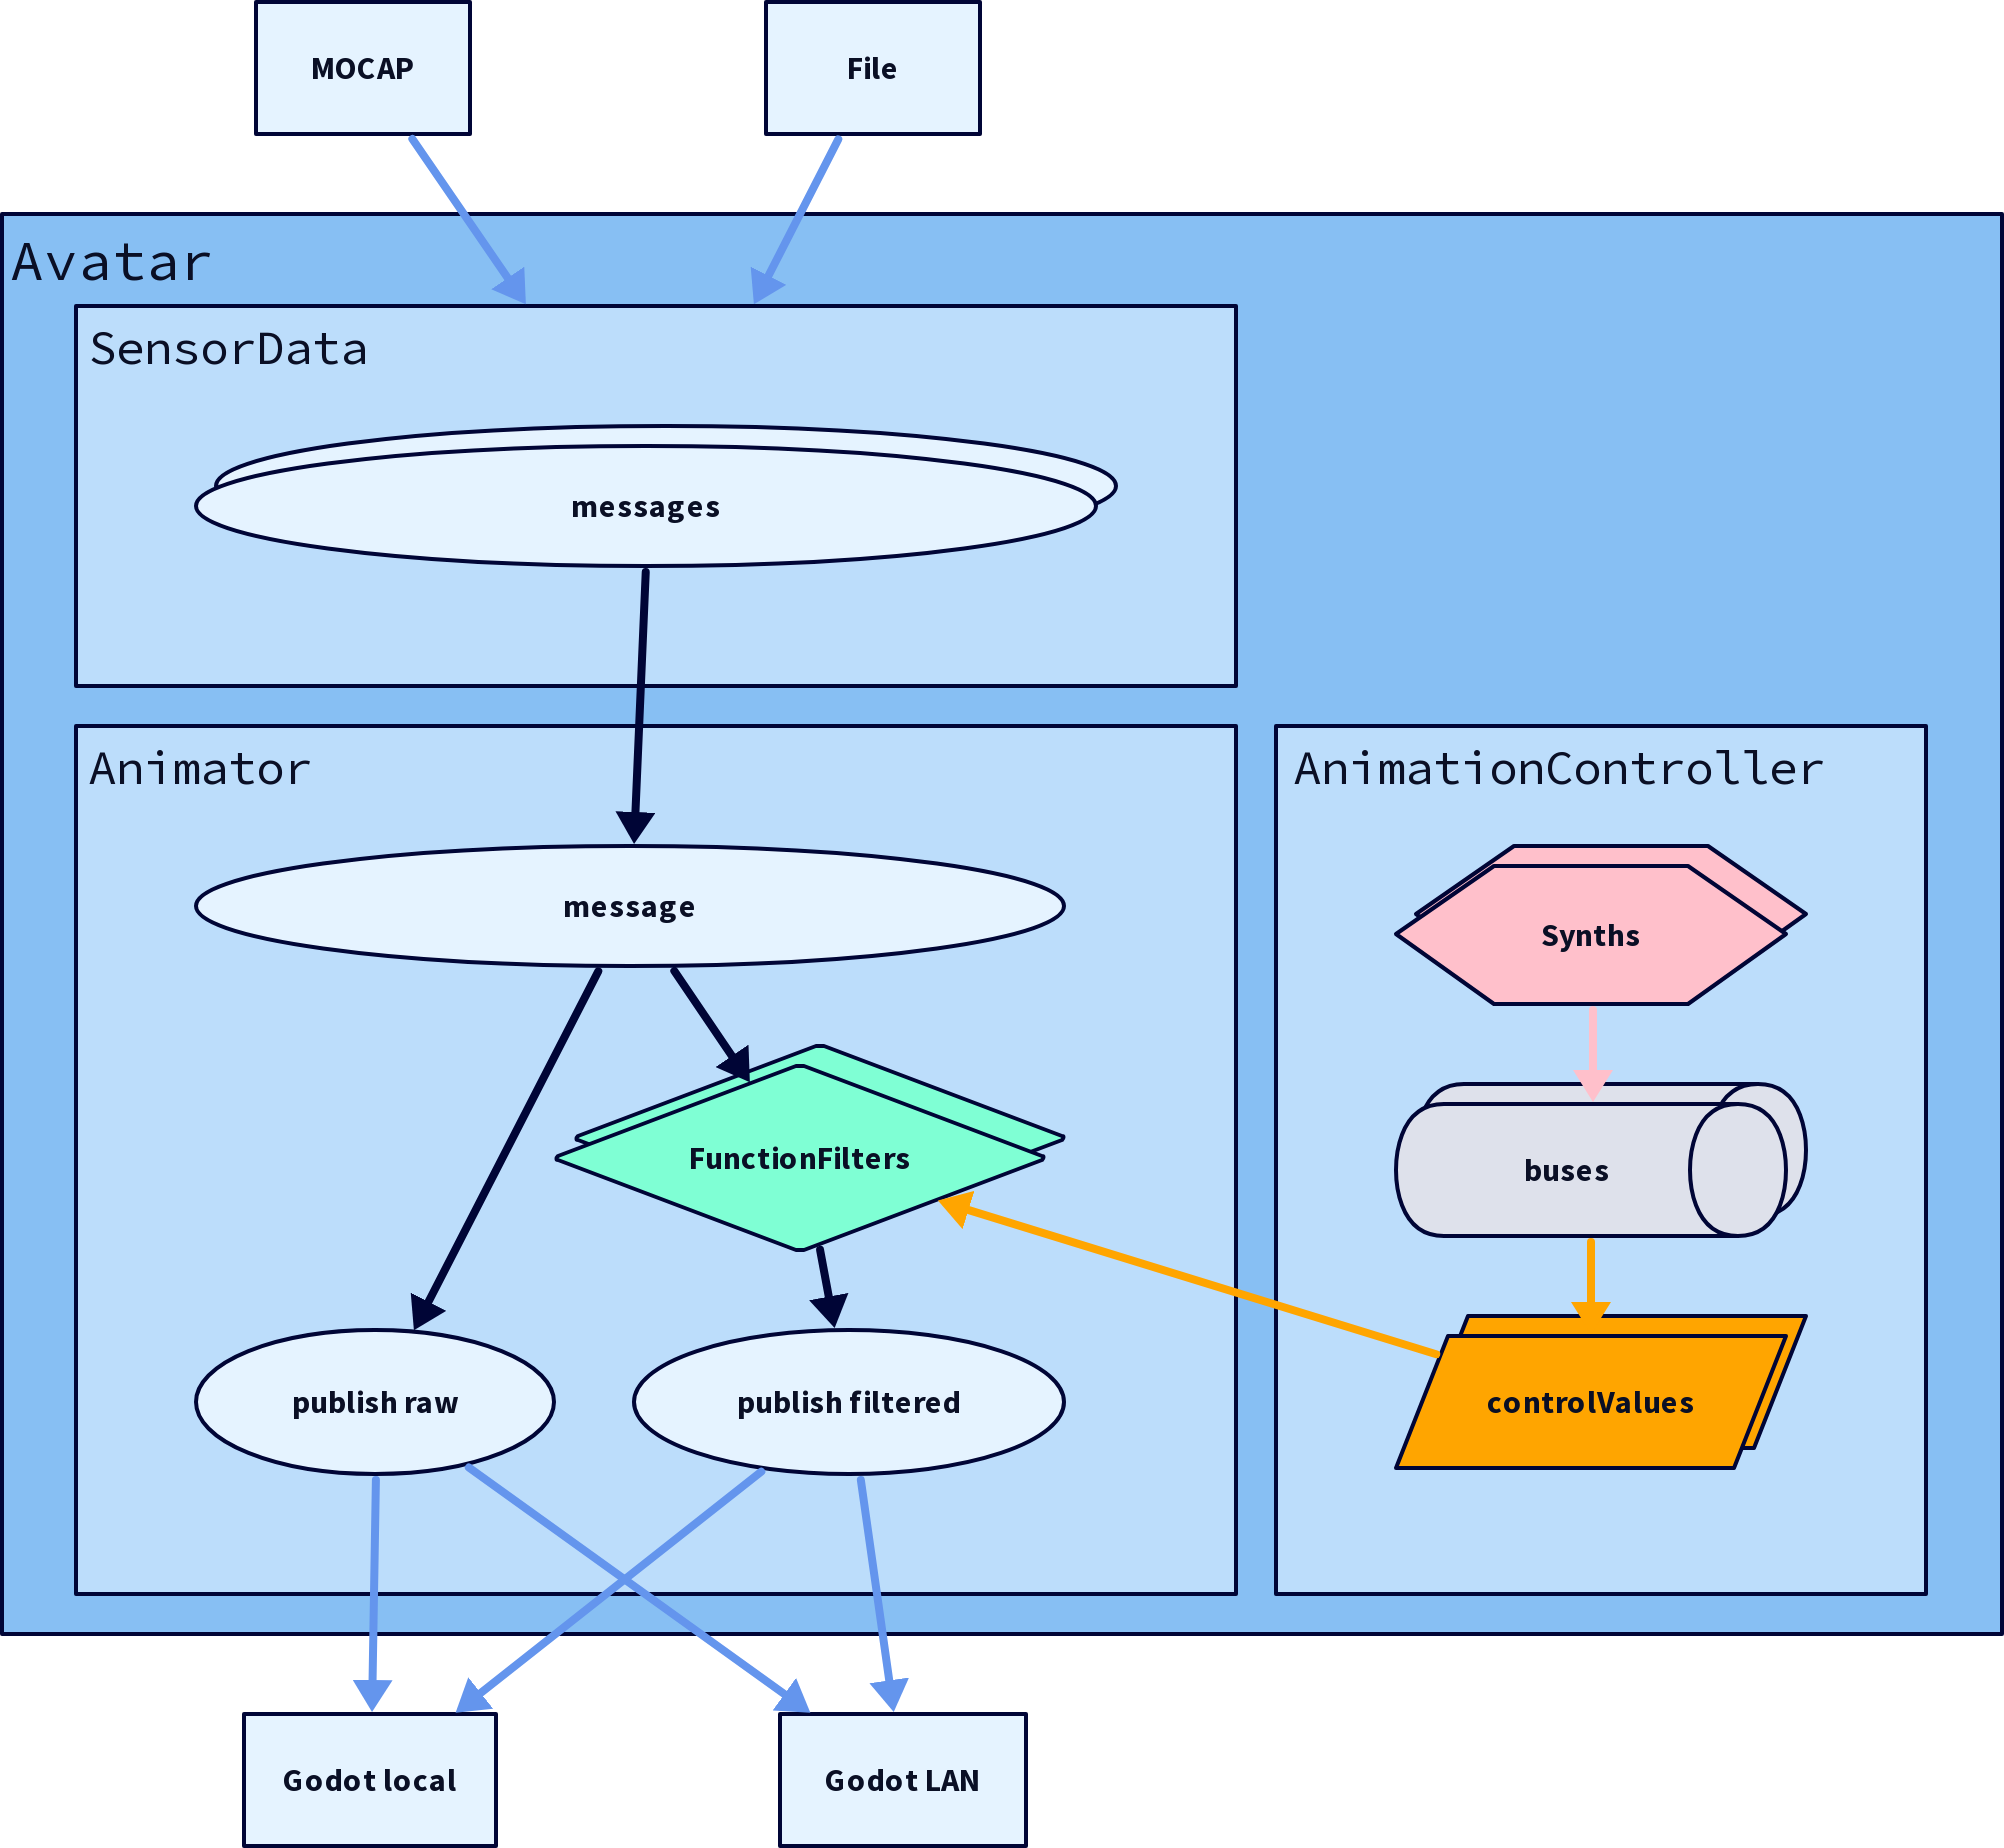
\includegraphics[width=.9\linewidth]{SC_messaging.png}
\end{center}

Following figure shows the mechanism for writing data from Synths to Buses in order to control animation and sound.

\begin{center}
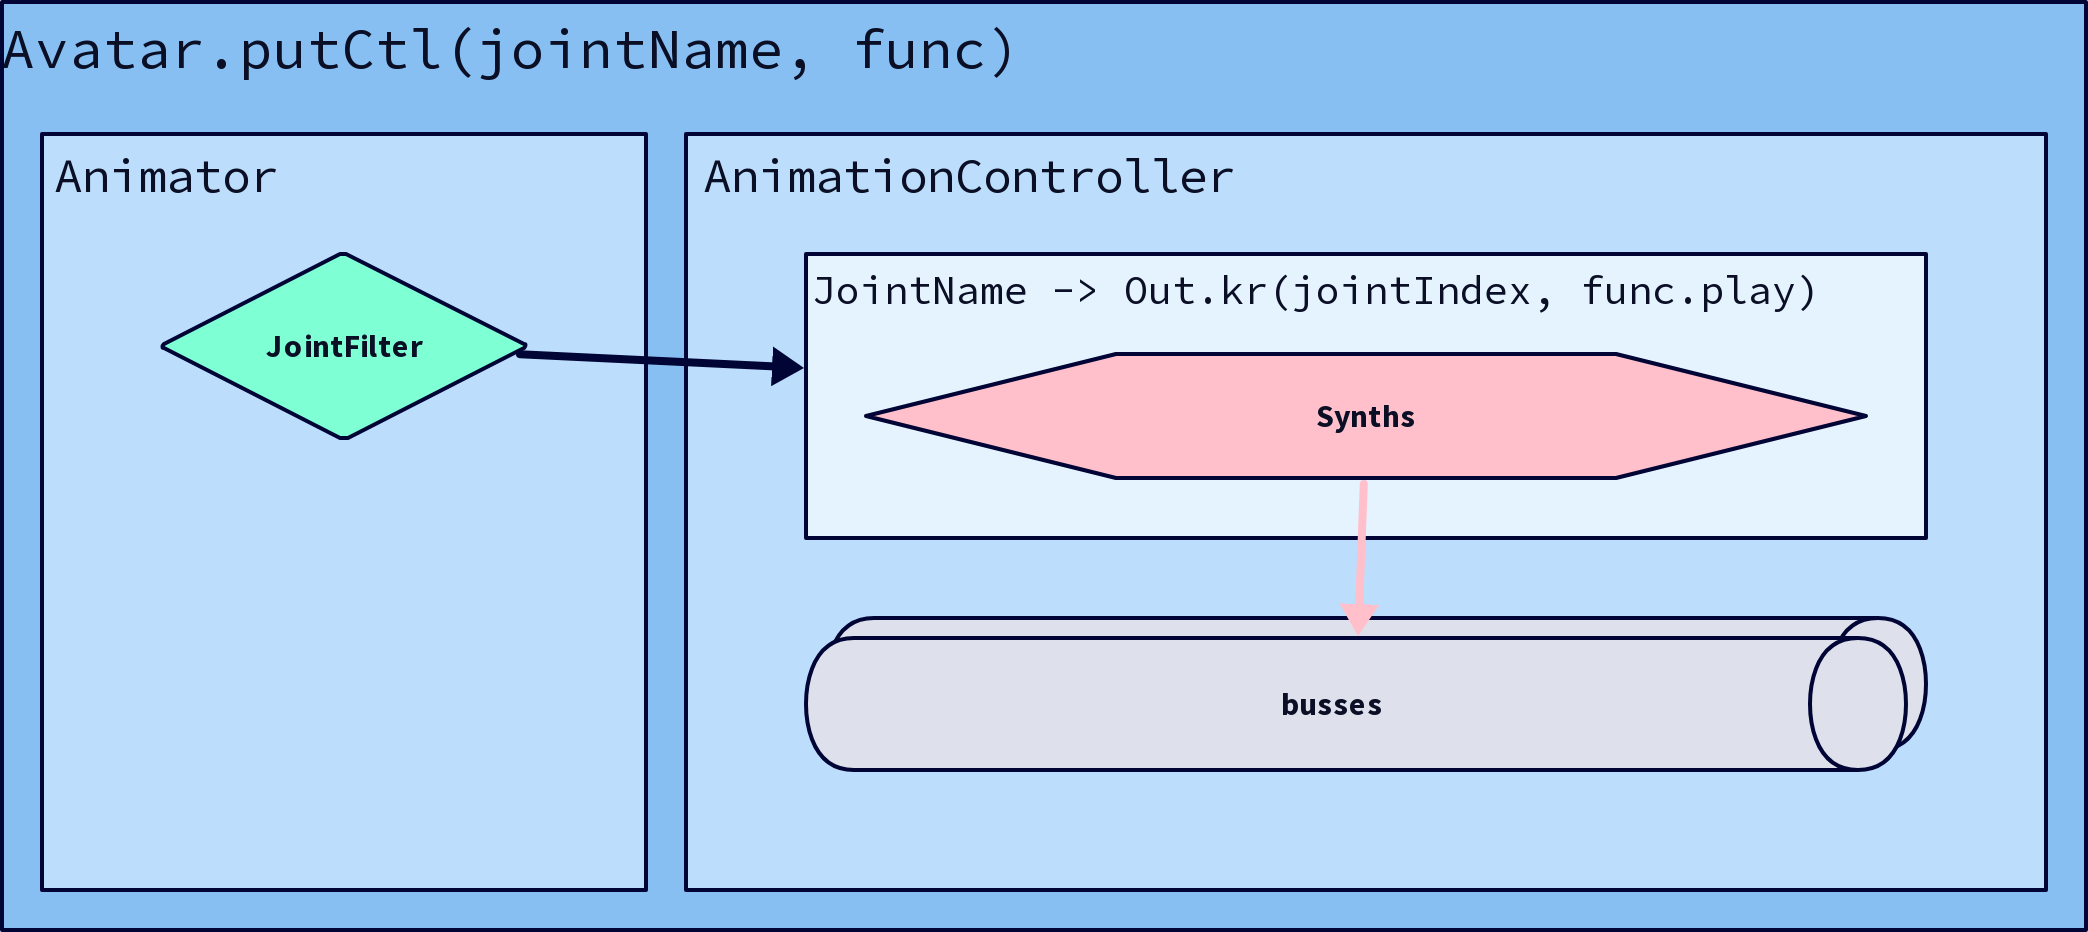
\includegraphics[width=.9\linewidth]{SC_writing_data_to_buses.png}
\end{center}
\section{Example Files}
\label{sec:org13a42e8}

The `sc-dance` library includes a `Guides` folder (and its subfolders) containing various example `.scd` files. These examples demonstrate different aspects of the library's functionality, from basic setup to advanced sound synthesis and animation control.

This section outlines the topics covered by these examples and suggests a logical progression for exploring the library.
\subsection{\textbf{Loading and Playing Animations}:}
\label{sec:org954f23f}
\begin{itemize}
\item How to load pre-recorded MOCAP session data.
\item Basic playback of animations in Godot.
\item Controlling animation speed and looping.
\end{itemize}
\subsection{\textbf{Modifying and Synthesizing Animations}:}
\label{sec:orgbb2e3fd}
\begin{itemize}
\item Applying filters to animation data (e.g., smoothing, scaling).
\item Real-time manipulation of joint data.
\item Creating custom animation behaviors.
\end{itemize}
\subsection{\textbf{Making Sound from Animation Data}:}
\label{sec:org8dc5387}
\begin{itemize}
\item Connecting animation parameters to sound synthesis (e.g., joint position to pitch, joint velocity to amplitude).
\item Using `slopePhrase` to extract meaningful control signals from motion.
\item Granular synthesis driven by animation data.
\item Triggering events based on animation thresholds.
\end{itemize}
\subsection{\textbf{Creating Avatars with Different Names and the Role of the Default Avatar}:}
\label{sec:orgd3c35c8}
\begin{itemize}
\item Instantiating multiple `Avatar` objects.
\item Managing and switching between active avatars.
\item Understanding the concept of the ``default'' avatar and its implications for global control.
\end{itemize}
\subsection{\textbf{Advanced Topics (Suggested Future Examples)}:}
\label{sec:org2db0916}
\begin{itemize}
\item Live MOCAP integration (if applicable).
\item Custom UGen development for animation processing.
\item Interfacing with other external software.
\item Building complex multi-avatar scenes.
\end{itemize}
\end{document}
